% !TEX encoding = UTF-8 Unicode
% -*- coding: UTF-8; -*-
% vim: set fenc=utf-8

\chapter{Abordagem para análise de rastros de proveniência}%
\label{chap:rastros-de-proveniencia}

Nesse capítulo é apresentado o Processador de Consultas (Query Processor), juntamente com a sua implementação e seus algoritmos. Além disso, aborda-se a relação entre os diversos tipos de rastros de proveniência existentes e a influência da seleção de um desses tipos na execução do QP.

Conforme abordado na \autoref{sec:rastreamento-de-dados-de-proveniencia}, o \textbf{rastreamento de dados de proveniência} em uma simulação computacional é realizado através do \textbf{mapeamento de atributos} de dados dos conjuntos de dados, sendo indispensável para tal. Reitera-se a definição de mapeamento de atributos da \autoref{subsec:mapeamento-de-atributos}, destacando que diz-se que existe um mapeamento de atributos entre dois atributos de dados \(da_1\) de um conjunto de dados \(ds_1\) e \(da_2\) de um conjunto de dados \(ds_2\), desde que ambos os atributos apresentem \((i)\) o mesmo identificador (nome) e \((ii)\) o mesmo tipo, e desde que \((iii)\) \(ds_1\) e \(ds_2\) sejam adjacentes no mesmo fluxo de dados, \textit{i.e.}, eles devem possuir uma transformação de dados em comum, sendo um deles a entrada e o outro a saída da mesma.

\section{Tipos de rastros de proveniência}%
\label{sec:tipos-de-rastros-de-proveniencia}

A fim de ilustrar as definições das próximas subseções, considere o fluxo de dados  \(D\ast\) da \autoref{fig:simple-dataflow-for-diff}, cujos atributos de dados \(A\ast\) estão listados na \autoref{tab:simple-attributes-for-diff}. 

\begin{figure}[htb]
    \centering
    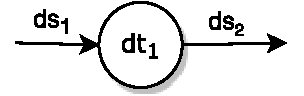
\includegraphics[width=0.4\textwidth]{img/simple-dataflow-for-diff}
    \caption[Exemplo de fluxo de dados para a seção \autoref{sec:tipos-de-rastros-de-proveniencia}]{Exemplo de fluxo de dados \(D\ast\) para a seção \autoref{sec:tipos-de-rastros-de-proveniencia}.}%
    \label{fig:simple-dataflow-for-diff}
\end{figure}

\begin{table}[htb]
    \centering
    \begin{tabular}{c|c|c}
    \textbf{Conjunto de dados} & \textbf{Nome do atributo} & \textbf{Tipo do atributo} \\ \hline
$ds_1$                        & $da_1$                        & inteiro                 \\
$ds_1$                        & $da_2$                        & booleano                \\
$ds_1$                        & $\textup{taskid\_}dt_1$      & inteiro                 \\ \hline
$ds_2$                        & $da_1$                        & inteiro                 \\
$ds_2$                        & $da_2$                        & inteiro                 \\
$ds_2$                        & $\textup{taskid\_}dt_1$      & inteiro                
    \end{tabular}
    \caption[Atributos de dados do fluxo de dados da \autoref{fig:simple-dataflow-for-diff}]{Atributos de dados \(A\ast\) do fluxo de dados \(D\ast\) da \autoref{fig:simple-dataflow-for-diff}.}
    \label{tab:simple-attributes-for-diff}
\end{table}

\subsection{Físico}%
\label{subsec:rastro-de-proveniencia-do-tipo-fisico}

O mapeamento de atributos de dados do \textbf{tipo físico} ocorre \emph{somente} entre pares de atributos de dados (de conjuntos de dados) especiais, que fazem parte de uma mesma tarefa (execução de uma transformação de dados) de uma mesma instância da simulação computacional, sendo denotadas por um identificador cujo nome é da forma \texttt{taskid\_\ast}, onde \ast{} representa um número arbitrário (\textit{i.e.}, um ou mais) de caracteres. O tipo desse atributo necessariamente deve ser um inteiro positivo. O propósito desse atributo é agrupar elementos de dados que foram processados em uma mesma instância de execução~/~tarefa de uma simulação computacional. No exemplo dessa seção, o mapeamento físico dos atributos de \(D\ast\) existe somente entre o par de atributos de dados \(ds_1.\textup{taskid\_}dt1\) e \(dt_2.\textup{taskid\_}dt1\), pois esses são os únicos atributos do tipo \textit{taskid} presentes em \(D\ast\).

\subsection{Lógico}

O mapeamento de atributos de dados do \textbf{tipo lógico} ocorre entre os \textbf{atributos de domínio} dos conjuntos de dados de uma simulação científica. Esses atributos de domínio necessariamente \emph{não} podem denotar o tipo \texttt{taskid} mencionado na subseção anterior. Sendo assim, o mapeamento lógico permite que as junções, regularmente realizadas pelos usuários ao desenvolver suas consultas, sejam expressas pelos mapeamentos lógicos de atributos. Consequentemente, assim como o mapeamento físico, o mapeamento lógico também pode reduzir o esforço necessário por parte do usuário ao desenvolver suas consultas, já que os principais relacionamentos entre conjuntos de dados poderiam ser representados~/~expressos pelos mapeamentos de atributos.

No exemplo dessa seção, o mapeamento lógico dos atributos de \(D\ast\) existe somente entre o par de atributos de dados \(ds_1.da_1\) e \(ds_2.da_1\). Note que \emph{não} existe mapeamento lógico entre \(ds_1.da_2\) e \(ds_2.da_2\) pois, apesar de possuírem o mesmo nome, esses atributos de dados possuem tipos de dados diferentes (inteiro e booleano). Além disso, o atributo \(taskid\textup{\_}dt1\) não foi considerado por ser específico do mapeamento físico.

\subsection{Híbrido}

Existe também cenários em que o usuário precise considerar os mapeamentos de atributos físico e lógico. Nesse cenário, o mapeamento de atributos de dados do \textbf{tipo híbrido} consiste na combinação --- ou, mais precisamente, na \emph{união} --- de ambos os tipos de mapeamentos de atributos anteriores: o físico e o lógico. 

Sendo assim, por meio da definição desses três tipos de mapeamentos de atributos, o usuário poderia especificar que tipos de relacionamentos são importantes de serem expressos~/~considerados ao realizar análises nos resultados obtidos em simulações computacionais. Esses relacionamentos, por exemplo, poderiam ser considerados ao longo de toda a simulação computacional (entre todos os relacionamentos entre transformações de dados) ou em determinadas transformações de dados.

Assim, no exemplo dessa seção, esse mapeamento envolve os seguintes atributos:

\begin{itemize}
    \item \(ds_1.da_1\) e \(ds_2.da_1\) (lógico); e
    \item \(ds_1.\textup{taskid\_}dt_1\) e \(ds_2.\textup{taskid\_}dt_1\) (físico).
\end{itemize}

\section{Desenvolvimento do Processador de Consultas}

Com o objetivo de permitir o desenvolvimento da abordagem para análise de rastros de proveniência em simulações computacionais, foi desenvolvido o \textbf{Query Processor}. Ele foi implementado na linguagem de programação Java, a qual foi escolhida pelas seguintes razões:

\begin{itemize}
    \item possui um bom suporte a orientação a objetos;
    \item está bastante consolidada no mercado e na academia, sendo uma escolha tradicional;
    \item facilita a integração do Query Processor com os outros componentes do DfAnalyzer, uma vez que eles também foram implementados originalmente em Java.
\end{itemize}

O projeto foi gerenciado e compilado pelo \texttt{Apache Maven~3.5.0}, tendo sido desenvolvido no ambiente de desenvolvimento integrado \texttt{NetBeans~8.2}, com a versão~1.8 do \texttt{JDK} (\textit{kit} de desenvolvimento) do \texttt{Java}. O banco de dados utilizado foi o \texttt{MonetDB~11.25.23}. O \texttt{git~2.11} foi utilizado como sistema de controle de versão distribuído para o projeto, o qual consiste de
% Linhas de código contadas com CLOC: https://github.com/AlDanial/cloc
22~arquivos-fonte~\texttt{*.java} e 23~classes, totalizando quase 2.000~linhas de código.

Além disso, para garantir a confiabilidade e a qualidade do projeto, 152~testes unitários foram implementados utilizando o \textit{framework} JUnit, distribuídos entre 15~arquivos-fonte.

\section{Algoritmos utilizados}%
\label{sec:algoritmos-utilizados}

Nessa seção serão abordados os principais algoritmos e funções utilizadas no Query Processor. Funções auxiliares referenciadas pelos mesmos estão definidas no \autoref{app:funcoes-auxiliares}. A notação utilizada é de pseudocódigo, e as definições dos algoritmos e nomes das variáveis utilizados foram ligeiramente alterados e simplificados em relação à implementação original, visando uma melhor clarificação e apresentação do código.

\subsection{Detecção das últimas transformações de dados}

Primeiramente, desenvolvemos um algoritmo para a detecção das últimas transformações de dados, a fim de que seja possível utilizar essas transformações para compreender melhor o encadeamento dos conjuntos de dados, conforme é apresentado nas próximas subseções. O \autoref{lst:algorithm-last-transformations} demonstra como obter as \textbf{últimas transformações de dados} \texttt{transformations} de um fluxo de dados \( D \), isto é, as transformações de dados \(dt\) as quais não possuem nenhuma outra transformação de saída após as mesmas. A ideia do algoritmo é bastante simples: basta checar todas as dependências de dados \( \phi \) --- do conjunto de dependência de dados do fluxo de dados \( D.\Phi \) --- cujo \( dt_{\textrm{next}} \) é nulo, e tomar o \( dt_{\textrm{previous}} \) das mesmas.

% https://tex.stackexchange.com/questions/73231/avoid-page-breaks-in-lstlistings
\begin{minipage}[c]{0.95\textwidth}
\begin{lstlisting}[language=pseudocode,label={lst:algorithm-last-transformations},caption={[Detecção das últimas transformações de dados]Detecção das útimas transformações de dados em uma especificação de fluxo de dados.}]
function getLastTransformations(%\(D\)%):
    transformations %\leftarrow% {}
    for each %\phi% %\in% %\(D.\Phi\)% do:
        if %$\phi.dt_{\texttt{next}} = \varnothing$% then:
            transformations %\leftarrow% transformations + 
        end if
    end do
    return transformations
end function
\end{lstlisting}
\end{minipage}

A complexidade de tempo do algoritmo é linear da ordem de \( O(\#(D.\Phi)) \), isto é, proporcional ao número de dependências de dados do fluxo de dados \( D \), e as transformações retornadas pelo algoritmo são armazenadas em uma simples lista encadeada, já que não é necessário acesso aleatório a essa estrutura de dados. Entretanto, na prática, com o objetivo de amortizar um pouco a complexidade, esse algoritmo é aplicado \textit{on-the-fly}, no momento em que o fluxo de dados é construído e instanciado no QP (\textit{c.f.} \autoref{subsec:preprocessamento}).

\subsection{Detecção das trilhas de transformações de dados}%
\label{subsec:deteccao-das-trilhas-de-transformacoes}

O \autoref{lst:algorithm-transformation-tracks} demonstra como obter as \textbf{trilhas de transformações de dados} \texttt{dtTracks} de um fluxo de dados \( D \). As trilhas são uma maneira natural de separar e agrupar transformações de dados em vários subconjuntos, definidos e limitados através de separações (do inglês, \textit{splits}) em \( D \). Tais separações existem no grafo do fluxo de dados em interseções de transformações que possuem mais de uma transformação de entrada ou de saída (\textit{i.e.}, grau do vértice maior do que 1). Por exemplo, na \autoref{fig:transformation-tracks}, podemos visualizar um exemplo de divisão e agrupamento de transformações de dados em trilhas.

\begin{figure}[htb]
    \centering
    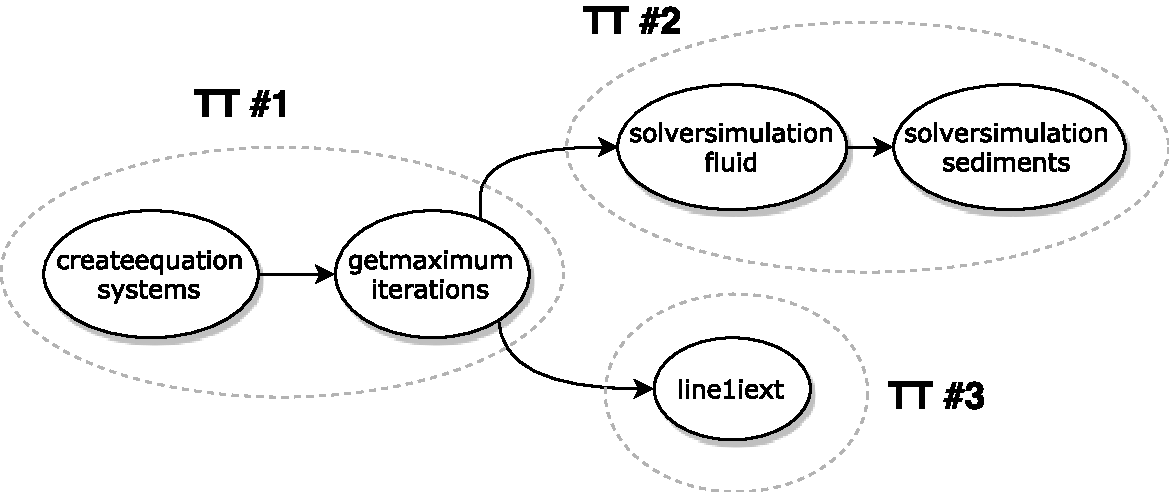
\includegraphics[width=\textwidth]{img/transformation-tracks}
    \caption[Exemplo de detecção das trilhas de transformações]{Exemplo de detecção das trilhas de transformações de dados de um fluxo de dados. Na figura existem três trilhas de transformações (\textsc{TT}).}%
    \label{fig:transformation-tracks}
\end{figure}

O algoritmo começa com as últimas transformações \texttt{lastDts} de \( D \) (encontradas no \autoref{lst:algorithm-last-transformations}), e caminha em direção às primeiras transformações de \( D \), utilizando uma estrutura de dados \texttt{queue} do tipo fila (FIFO - \textit{First In First Out}) como armazenamento temporário das próximas transformações de dados a serem analisadas. A ideia principal é realizar a detecção do fim --- e, consequentemente, também do início --- de cada trilha de transformação \texttt{dtTrack}, que pode acontecer em várias situações: \textit{e.g.}, sempre que o grau de saída do vértide de uma transformação for maior do que 1, indicando que a transformação em questão possui várias transformações de saída.

\begin{minipage}[c]{0.95\textwidth}
\begin{lstlisting}[language=pseudocode,label={lst:algorithm-transformation-tracks},caption={[Detecção das trilhas de transformações]Detecção do rastro do fluxo de dados no nível de trilhas de transformações.}]
function getTransformationTracks(%\(D\)%):
    dtTracks %\leftarrow% {}
    lastDts %\leftarrow% getLastTransformations(%\(D\)%)%~\quad%#%~\autoref{lst:algorithm-last-transformations}%
    queue %\leftarrow% {}%~\quad%#%~%FIFO (First In First Out)
    queue.enqueue(lastDts)
    while queue is not empty do:
        dt %\leftarrow% queue.dequeue()
        nextDts %\leftarrow% getNextTransformations(%\(D\)%, dt)
        if dt %\in% lastDts
           or hasManyOutputDatasets(%\(D\)%, dt)
           or hasManyNextTransformations(%\( D \)%, dt)
           or anyTransformationHasManyInputDatasets(%\(D\)%, nextDts)
           then:
            dtTrack %\leftarrow% {dt}
            dtTracks %\leftarrow% dtTracks + {dtTrack}
        else then:
            dtTrack %\leftarrow% getTransformationTrack(dtTracks, nextDts[0])
            dtTrack %\leftarrow% dtTrack + {dt}
        end if
        previousDts %\leftarrow% getPreviousTransformations(%\(D\)%, dt)
        queue.enqueue(previousDts)
    end do
    return dtTracks
end function
\end{lstlisting}
\end{minipage}

A complexidade de tempo do algoritmo é linear da ordem de \( O(\#(D.\Phi)) \), como no \autoref{lst:algorithm-last-transformations}. As trilhas de transformações \texttt{dtTracks} são armazenadas em listas encadeadas de transformações --- acesso aleatório não é necessário, porém convém armazená-las na mesma ordem em que foram encontradas.

\subsection{Detecção das trilhas de conjuntos de dados}

O \autoref{lst:algorithm-dataset-tracks} tem como função obter as \textbf{trilhas de conjuntos de dados} \texttt{dsTracks} de um fluxo de dados \( D \). O conceito de trilha de conjuntos de dados é análogo e baseado no de trilha de transformações de dados, mencionado na \autoref{subsec:deteccao-das-trilhas-de-transformacoes}: é uma forma de dividir e agrupar conjuntos de dados em diversos subconjuntos.

O algoritmo funciona com base no \autoref{lst:algorithm-transformation-tracks}: uma vez tomadas as trilhas de transformações de dados \texttt{dtTracks}, é simples obter cada uma das trilhas de conjuntos de dados \texttt{dsTrack} a partir de cada \texttt{dtTrack}. Para isso, basta tomar a união de todos os conjuntos de dados adjacentes (\textit{i.e.} anteriores e posteriores) a todas as transformações de dados de \texttt{dtTrack}.

\begin{minipage}[c]{0.95\textwidth}
\begin{lstlisting}[language=pseudocode,label={lst:algorithm-dataset-tracks},caption={[Detecção das trilhas de conjuntos de dados]Detecção do rastro do fluxo de dados no nível de trilhas de conjuntos de dados.}]
function getDatasetTracks(%\(D\)%):
    dsTracks %\leftarrow% {}
    dtTracks %\leftarrow% getTransformationTracks(D)%~\quad%#%~\autoref{lst:algorithm-transformation-tracks}%
    for each dtTrack %\in% dtTracks do:
        dsTrack %\leftarrow% {}
        for each dt %\in% dtTrack do:
            if dsTrack is empty then:
                dsTrack %\leftarrow% dsTrack + {getNextDatasets(%\(D\)%, dt)}
            end if
            dsTrack %\leftarrow% dsTrack + {getPreviousDatasets(%\(D\)%, dt)}
        end do
        dsTracks %\leftarrow% dsTracks + {dsTrack}
    end do
    return dsTracks
end function
\end{lstlisting}
\end{minipage}

A complexidade de tempo do algoritmo é a mesma do algoritmo do \autoref{lst:algorithm-transformation-tracks}: linear da ordem de \( O(\#(D.\Phi)) \), e as trilhas de conjuntos de dados \texttt{dsTracks} são também armazenadas em listas encadeadas de conjuntos de dados.

\subsection{Obtenção de múltiplos mapeamentos de atributos entre dois conjuntos de dados}

O \autoref{lst:algorithm-attribute-mappings} demonstra como obter \textbf{múltiplos mapeamentos de atributos} entre dois conjuntos de dados \(ds_{\textup{input}}\) e \(ds_{\textup{output}}\). Assume-se que ambos os conjuntos de dados sejam adjacentes, compartilhando uma mesma transformação de dados \texttt{dt} em comum, de modo que um desses conjuntos de dados é consumido e o outro é produzido pela mesma. Além disso, como mencionado na \autoref{sec:tipos-de-rastros-de-proveniencia}, esses mapeamentos de atributos podem ser de três tipos (variável \texttt{type} no pseudo-código): lógico, físico e híbrido.

\begin{minipage}[c]{0.95\textwidth}
\begin{lstlisting}[language=pseudocode,label={lst:algorithm-attribute-mappings},caption={[Obtenção de múltiplos mapeamentos de atributos]Obtenção de múltiplos mapeamentos de atributos entre dois conjuntos de dados adjacentes.}]
function getAttributesMapping(dt,%\(ds_{\textrm{input}}\)%,%\(ds_{\textrm{output}}\)%,type)
   attrs %\leftarrow% {}
   if type %\in% {physical, hybrid} then:
       attrs %\leftarrow% attrs + {t.getTaskIdAttribute()}
   end if
   if type %\in% {logical, hybrid} then:
       for each inAttr %\in% %\(ds_{\textrm{input}}\).A% do:
           for each outAttr %\in% %\(ds_{\textrm{output}}\).A% do:
               if inAttr.name = outAttr.name
                  and inAttr.type = outAttr.type then:
                   attrs %\leftarrow% attrs + {inAttr}
               end if
           end do
       end do
   end if
   return attrs
end function
\end{lstlisting}
\end{minipage}

\begin{itemize}
    \item No caso do mapeamento de atributos do tipo \emph{lógico}, o algoritmo itera sobre o produto cartesiano entre os atributos dos dois conjuntos de dados. Para cada par desses atributos, verifica-se se: \((i)\) eles possuem o mesmo identificador (nome) e se \((ii)\) eles possuem o mesmo tipo; caso positivo para ambos, diz-se que esse par de atributos possui um mapeamento lógico, o qual é armazenado em uma lista encadeada retornada pelo algoritmo.

    \item No caso do mapeamento de atributos do tipo \emph{físico}, o único atributo que é levado em conta entre os dois conjuntos de dados é o \textit{task id} da transformação de dados \texttt{dt} associada a ambos, responsável por identificar a proveniência retrospectiva da simulação computacional.

    \item Por fim, o mapeamento do tipo \emph{híbrido} engloba a união de todos os atributos dos mapeamentos lógico e físico.
\end{itemize}

A complexidade computacional do algoritmo é da ordem do produto do número de atributos de cada conjunto de dados: \(O(\#(ds_{\textup{input}}.A) \times \#(ds_{\textup{output}}.A))\), e os mapeamentos de atributos são armazenados em listas encadeadas.

\subsection{Obtenção dos caminhos entre dois conjuntos de dados}

A função \texttt{findPaths} do \autoref{lst:algorithm-find-paths} inicializa a estrutura de estados \texttt{state}, necessária para a chamada da função de busca em profundidade \abbrev{DFS}{Depth-first Search (Busca em profundidade)} \texttt{depthFirstSearch} (DFS) do \autoref{lst:algorithm-dfs}. Essas duas funções atuam em conjunto com um objetivo em comum: \textbf{obter todos os caminhos entre dois conjuntos de dados} \texttt{dsOrigin} e \texttt{dsDestination} do fluxo de dados \(D\).
Nesse contexto, um caminho é definido como uma lista ordenada de conjuntos de dados, cujo primeiro elemento é \texttt{dsOrigin}, e cujo último elemento é \texttt{dsDestination}.

Como podem existir potencialmente vários caminhos entre esse par de conjuntos de dados, a função \texttt{findPaths} possui dois argumentos adicionais que atuam como filtros:

\begin{itemize}
    \item \texttt{dsIncludes} --- uma coleção de conjuntos de dados: todos eles devem estar presentes no caminho para que tal caminho seja retornado pela função \texttt{findPaths};
    \item \texttt{dsExcludes} --- o oposto de \texttt{dsIncludes}: nenhum dos caminhos que fazem parte da coleção \texttt{dsExcludes} pode estar presente nos caminhos retornados por \texttt{findPaths}.
\end{itemize}

\begin{minipage}[c]{0.95\textwidth}
\begin{lstlisting}[language=pseudocode,label={lst:algorithm-find-paths},caption={[Obtenção dos caminhos entre dois conjuntos de dados]Obtenção de todos os caminhos entre dois conjuntos de dados, inicializando a \textsc{DFS} com um estado inicial apropriado.}]
function findPaths(D,dsOrigin,dsDestination,dsIncludes,dsExcludes)
    state %\leftarrow% {}
    state.visited %\leftarrow% {dsOrigin}
    state.paths %\leftarrow% {}
    state.dsOrigin = dsOrigin
    state.dsDestination = dsDestination
    state.dsIncludes = dsIncludes
    state.dsExcludes = dsExcludes
    depthFirstSearch(D,state)%~\quad%#%~\autoref{lst:algorithm-dfs}%
    return state.paths
end function
\end{lstlisting}
\end{minipage}

\begin{minipage}[c]{0.95\textwidth}
\begin{lstlisting}[language=pseudocode,label={lst:algorithm-dfs},caption={[Busca em Profundidade (DFS) dos caminhos]Depth First Search (DFS): busca em profundidade de todos os caminhos entre dois conjuntos de dados.}]
function depthFirstSearch(D,state)
    nodes %\leftarrow% getNextDatasets(D,state.visited.getLast())
    for each node %\in% nodes do:
        if node %\in% state.visited then:
            continue
        end if
        if node = state.dsDestination then:
            state.visited %\leftarrow% state.visited + {node}
            path %\leftarrow% new Path(state.visited)
            if state.dsIncludes %\in% path and state.dsExcludes%~%%\not\in%%~%path then:
                state.paths %\leftarrow% state.paths + {path}
            end if
            state.visited.pop()
            break
        end if
    end do
    for node %\in% nodes do:
        if node %\in% state.visited or node = state.dsDestination then:
            continue
        end if
        state.visited %\leftarrow% state.visited + {node}
        depthFirstSearch(D,state)
        state.visited.pop()
    end do
end function
\end{lstlisting}
\end{minipage}

A função \texttt{depthFirstSearch} é responsável por realizar uma busca no grafo do fluxo de dados \(D\), tratando cada conjunto de dados como um vértice do grafo. Dois vértices são considerados adjacentes se existe uma transformação de dados que consome um dos vértices e produz o outro. A DFS opera recursivamente, utilizando a estrutura \texttt{state} para salvar dados intermediários durante a busca, e também para popular a coleção \texttt{state.paths} com os caminhos encontrados. A coleção de conjuntos de dados \texttt{state.visited} armazena os conjuntos de dados que já foram processados, a fim de evitar que a busca seja executada indefinidamente.

A complexidade computacional desse par de funções (\texttt{findPaths} e \texttt{depthFirstSearch}) é da ordem de \(O(\#(S) + \#(T))\), que é a complexidade computacional da DFS\footnote{\textbf{Observação:} a complexidade computacional da função \texttt{getNextDatasets} é de $O(\#(D.\Phi)^2)$. No entanto, como existe um pré-processamento das estruturas de dados (\textit{c.f.} \autoref{subsec:preprocessamento}), podemos desprezar essa complexidade, levando em conta apenas o resultado originalmente obtido.}. Os caminhos encontrados são armazenados em uma lista encadeada.

\subsection{Geração da consulta em SQL}%
\label{subsec:geracao-da-consulta-em-sql}

O \autoref{lst:algorithm-generate-sql-query} é uma versão simplificada do algoritmo responsável pela \textbf{geração da consulta na linguagem SQL} a partir das especificações providas pelo usuário. A assinatura da função possui os seguintes argumentos:

\begin{itemize}
    \item \texttt{D}: o fluxo de dados a ser analisado;
    \item \texttt{dsOrigins}: os conjuntos de dados que serão usados como origem na busca de caminhos do \autoref{lst:algorithm-find-paths};
    \item \texttt{dsDestinations}: os conjuntos de dados que serão usados como destino na busca de caminhos do \autoref{lst:algorithm-find-paths}. Um produto cartesiano entre \texttt{dsDestinations} e \texttt{dsOrigins} é realizado, gerando todos os pares possíveis entre cada conjunto de dados dessas coleções, cada um dos quais são utilizados na busca de caminhos;
    \item \texttt{type}: o tipo de mapeamento de atributos que será utilizado na especificação das seleções em SQL, conforme abordado na \autoref{sec:tipos-de-rastros-de-proveniencia} e no \autoref{lst:algorithm-attribute-mappings}.
    \item \texttt{projections}: especificação das projeções pelo usuário, optando por quais atributos devem ser incluídos na cláusula \textsc{SELECT} do SQL;
    \item \texttt{selections}: especificação das seleções pelo usuário, optando por quais condições devem ser incluídas na cláusula \textsc{WHERE} do SQL.
    \item \texttt{dsIncludes}: utilizado como filtro para o \autoref{lst:algorithm-find-paths}; somente os caminhos contendo \emph{todos} os conjuntos de dados especificados nessa coleção serão utilizados na consulta;
    \item \texttt{dsExcludes}: o oposto do item anterior; somente os caminhos que não contêm \emph{nenhum} dos conjuntos de dados especificados nessa coleção serão utilizados na consulta; é utilizado como filtro para o \autoref{lst:algorithm-find-paths}.
\end{itemize}

\begin{minipage}[c]{0.95\textwidth}
\begin{lstlisting}[language=pseudocode,label={lst:algorithm-generate-sql-query},caption={[Geração da consulta em SQL]Geração da consulta na linguagem SQL a partir das especificações do usuário.}]
function generateSqlQuery(D,dsOrigins,dsDestinations,type,
projections,selections,dsIncludes, dsExcludes)
    selectClause %\leftarrow% {}
    fromClause   %\leftarrow% {}
    whereClause  %\leftarrow% {}
    for each projection %\in% projections do:
        selectClause %\leftarrow% selectClause + {projection}
    end do
    for each selection %\in% selections do:
        whereClause %\leftarrow% whereClause + {selection}
    end do
    for each dsOrigin %\in% dsOrigins do:
        for each dsDestination %\in% dsDestinations do:
            paths %\leftarrow% findPaths(dsOrigin, dsDestination, dsIncludes, dsExcludes)%~\quad%#%~\autoref{lst:algorithm-find-paths}%
            for each path %\in% paths do:
                for each ds %\in% path do:
                    fromClause %\leftarrow% fromClause + {ds}
                end do                
                for (i %\leftarrow% 1; i < path.size(); i %\leftarrow% i + 1) do:
                    prevDs %\leftarrow% path[i - 1]
                    nextDs %\leftarrow% path[i]
                    attrMapping %\leftarrow% getAttributesMapping(getTransformation(D, prevDs,nextDs),prevDs,nextDs, type)%~\quad%#%~\autoref{lst:algorithm-attribute-mappings}%
                    for each attr %\in% attrMapping do:
                        whereClause.addSelection(prevDs.attr, "=", nextDs.attr)
                        if projections is empty then:
                            selectClause %\leftarrow% selectClause + {prevDs.attr, rightDs.attr}
                        end if
                    end do
                end do
            end do
        end do
    end do
    sqlQuery %\leftarrow% new SqlQuery(selectClause, fromClause, whereClause)
    return sqlQuery
end function
\end{lstlisting}
\end{minipage}

O algoritmo do \autoref{lst:algorithm-generate-sql-query} torna-se simples, desde que delega as tarefas mais complexas para o \texttt{findPaths} (\autoref{lst:algorithm-find-paths}) e para o \texttt{getAttributesMapping} (\autoref{lst:algorithm-attribute-mappings}). Em princípio, todos os caminhos entre cada par do produto cartesiano entre os conjuntos de dados de origem \texttt{dsOrigins} e os de saída \texttt{dsDestinations} são encontrados. Então, para cada caminho, os mapeamentos de atributos entre cada par de conjuntos de dados adjacentes do mesmo são determinados e anotados.

Depois, são definidas cada uma das cláusulas fundamentais da linguagem SQL: \textsc{SELECT}, \textsc{FROM} e \textsc{WHERE}, as quais passam a ser populadas, uma a uma, através dos algoritmos e estruturas de dados apresentados anteriormente:

\begin{itemize}
    \item a cláusula \textsc{FROM} é populada automaticamente e não-extensivamente incluindo, par fins de performance, \emph{somente} as tabelas (atributos de conjuntos de dados) necessárias para a apresentação dos resultados da consulta ao usuário;
    \item a cláusula \textsc{SELECT} é populada de acordo com a especificação do usuário no argumento \texttt{projections}: uma vez que é o usuário quem deve escolher quais atributos ele deseja visualizar e consultar, o algoritmo não interfere de forma alguma nessa cláusula. No entanto, para fins de usabilidade, caso o usuário não especifique nenhuma projeção de atributo, o algoritmo popula a cláusula automaticamente e extensivamente, utilizando todos os atributos mapeados entre todo par de conjuntos de dados especificados como origem e destino (em \texttt{dsOrigins} e \texttt{dsDestinations}, respectivamente);
    \item finalmente, a cláusula \textsc{WHERE} é a mais importante do ponto de vista de análise de rastros de proveniência, uma vez que é ela quem atua como filtro~/~seleção, limitando a consulta somente aos dados que realmente satisfazem a especificação do usuário. Desse modo, ela é populada automaticamente pelo algoritmo, inclusive com todos os mapeamentos de atributos (físico, lógico ou híbrido, dependendo do valor da variável \texttt{type}) encontrados nos caminhos entre o produto cartesiano de \texttt{dsOrigins} e \texttt{dsDestinations}. Além da população implícita e automática pelo algoritmo, o usuário também pode especificar seleções adicionais a serem incluídas nessa cláusula através da variável \texttt{selections}.
\end{itemize}

\subsection{Pré-processamento}%
\label{subsec:preprocessamento}

Os algoritmos apresentados anteriormente possuem, \emph{em geral}, uma complexidade computacional de \textbf{ordem linear} em relação ao número de conjuntos de dados, de transformações de dados, de dependências de dados ou de atributos de dados, dependendo do algoritmo e da função auxiliar utilizada. Isso se deve ao fato de que a maioria das estruturas de dados empregadas inicialmente é do tipo lista encadeada, e os laços presentes nos algoritmos usualmente iteram sobre toda a lista em questão. Além disso, existem algumas funções como a presente no \autoref{lst:get-next-datasets-2} que possuem complexidade computacional da \textbf{ordem quadrática} em relação ao número de dependências de dados presentes no fluxo de dados.

Uma vez que um dos principais interesses do Query Processor é a aplicação do mesmo em simulações computacionais de larga escala, que incluem potencialmente uma quantidade enorme de dependências de dados e de atributos de dados, torna-se necessário melhorar o seu desempenho, não se limitando por algoritmos de ordem quadrática de complexidade temporal.

A fim de resolver esse problema, diversas \textbf{otimizações de pré-processamento de dados e de metadados} foram empregadas e computadas, efetivamente diminuindo a complexidade computacional dos algoritmos anteriores e das funções auxiliares utilizadas neles, trocando tempo por espaço / armazenamento. Na prática, isso significa o seguinte:

\begin{enumerate}
    \item as \emph{próximas} transformações de dados e os \emph{próximos} conjuntos de dados de cada conjunto de dados e de cada transformação de dados foram computadas no instante da instanciação do fluxo de dados, tendo sido armazenados em \textit{HashMultimaps}\footnote{\textit{HashMultimap} é uma estrutura de dados da biblioteca Guava da Google (\url{https://github.com/google/guava}) que provê armazenamento e consulta de pares de dados chave e valor em uma \textit{hashtable}.};
    \item analogamente, as transformações de dados \emph{anteriores} e os conjuntos de dados \emph{anteriores} também foram pré-computados;
    \item as últimas transformações de dados (\autoref{lst:algorithm-last-transformations}), as trilhas de transformações de dados (\autoref{lst:algorithm-transformation-tracks}) e as trilhas de conjuntos de dados (\autoref{lst:algorithm-dataset-tracks}) foram computadas uma única vez, e então permanentemente armazenadas para uso posterior --- em vez de, por exemplo, serem recomputadas a cada referência às mesmas.
\end{enumerate}

Os itens 1 e 2 eliminam completamente a necessidade de iteração sobre as dependências de dados, eliminando a complexidade computacional de ordem quadrática dos algoritmos, aumentando significativamente a performance dos mesmos. O item 3 emprega uma técnica chamada \textit{memoization}, que evita computar mais de uma vez o mesmo dado: os acessos após o primeiro são realizados em \(O(1)\). Essas otimizações de pré-processamento, pré-computação e \textit{memoization} foram fundamentais para garantir uma boa performance para o Query Processor.

\section{Um exemplo de consulta}%
\label{sec:um-exemplo-de-consulta}

Para ilustrar uma consulta utilizando o \autoref{lst:algorithm-generate-sql-query} (\texttt{generateSqlQuery}), vamos considerar como exemplo o fluxo de dados \(D^{\prime}\) da \autoref{fig:example-query-dataflow}, cujos atributos estão listados na \autoref{tab:example-query-attributes} e cujos elementos de dados estão listados na \autoref{tab:example-query-data-elements}.

\begin{figure}[!htb]
    \centering
    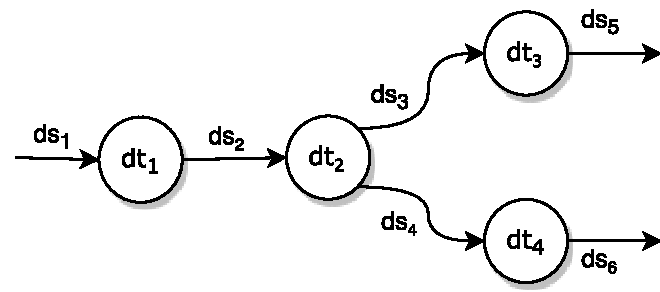
\includegraphics[width=\textwidth]{img/example-query-dataflow}
    \caption[Fluxo de dados de exemplo]{Fluxo de dados \(D^{\prime}\) utilizado como exemplo para a \autoref{sec:um-exemplo-de-consulta}.}%
    \label{fig:example-query-dataflow}
\end{figure}

\begin{table}[!htb]
    \centering
    \begin{tabular}{c|c|c}
    \textbf{Conjunto de dados} & \textbf{Nome do atributo} & \textbf{Tipo do atributo} \\ \hline
$ds_1$                        & $da_1$                        & inteiro                 \\
$ds_1$                        & $da_2$                        & booleano                \\
$ds_1$                        & $\textup{taskid\_}dt_1$      & inteiro                 \\ \hline
$ds_2$                        & $da_1$                        & inteiro                 \\
$ds_2$                        & $da_2$                        & inteiro                 \\
$ds_2$                        & $\textup{taskid\_}dt_1$      & inteiro                 \\
$ds_2$                        & $\textup{taskid\_}dt_2$      & inteiro                 \\ \hline
$ds_4$                        & $da_3$                        & string                  \\
$ds_4$                        & $\textup{taskid\_}dt_2$      & inteiro                  
    \end{tabular}
    \caption[Atributos de dados do fluxo de dados \(D^{\prime}\)]{Atributos de dados do fluxo de dados \(D^{\prime}\).}
    \label{tab:example-query-attributes}
\end{table}

\begin{table}[!htb]
    \centering
    \begin{tabular}{|c|c|c|c|c|}
\hline
\textbf{ds\textsubscript{1}} & \textbf{da\textsubscript{1}}    & \textbf{da\textsubscript{2}}    & \multicolumn{2}{c|}{\textbf{taskid\_dt\textsubscript{1}}}   \\ \hline
$de_1$          & 100             & verdadeiro      & \multicolumn{2}{c|}{1}                      \\
$de_2$          & 200             & falso           & \multicolumn{2}{c|}{1}                      \\
$de_3$          & 300             & verdadeiro      & \multicolumn{2}{c|}{2}                      \\ \hline
\textbf{ds\textsubscript{2}} & \textbf{da\textsubscript{1}}    & \textbf{da\textsubscript{2}}    & \textbf{taskid\_dt\textsubscript{1}} & \textbf{taskid\_dt\textsubscript{2}} \\ \hline
$de_1$          & 100             & -20             & 1                    & 1                    \\
$de_2$          & 200             & -45             & 1                    & 2                    \\
$de_3$          & 300             & 42              & 2                    & 2                    \\ \hline
\textbf{ds\textsubscript{4}} & \multicolumn{2}{c|}{\textbf{da\textsubscript{3}}} & \multicolumn{2}{c|}{\textbf{taskid\_dt\textsubscript{2}}}   \\ \hline
$de_1$          & \multicolumn{2}{c|}{alpha}        & \multicolumn{2}{c|}{1}                      \\
$de_2$          & \multicolumn{2}{c|}{bravo}        & \multicolumn{2}{c|}{2}                      \\
$de_3$          & \multicolumn{2}{c|}{charlie}      & \multicolumn{2}{c|}{2}                      \\ \hline
    \end{tabular}
    \caption[Elementos de dados do fluxo de dados \(D^{\prime}\)]{Elementos de dados do fluxo de dados \(D^{\prime}\).}
    \label{tab:example-query-data-elements}
\end{table}

\subsection{Exemplo~\#1}

Como segundo exemplo, considere a consulta envolvendo os conjuntos de dados $ds_1$ como origem e $ds_2$ como destino, especificada na \autoref{tab:example-query-arguments-2}. que gera o código em SQL apresentado no \autoref{lst:example-query-output-2}. Os resultados obtidos pela consulta em SQL podem ser observados na \autoref{tab:example-query-results-2}.

\begin{table}[!htb]
    \centering
    \begin{tabular}{c|c}
\textbf{Argumento}          & \textbf{Valor} \\ \hline
\texttt{D}                  & \(D^{\prime}\) \\
\texttt{dsOrigins}          & \(\{ds_{1}\}\) \\
\texttt{dsDestinations}     & \(\{ds_{2}\}\) \\
\texttt{type}               & physical       \\
\texttt{projections}        & \{$ds_{1}.da_{1}$, $ds_{1}.da_{2}$, $ds_{2}.da_{2}$\}    \\
\texttt{selections}         & \varnothing \\
\texttt{dsIncludes}         & \varnothing    \\
\texttt{dsExcludes}         & \varnothing    \\
\end{tabular}
\caption[Argumentos da função \texttt{generateSqlQuery} para o Exemplo \#2]{Argumentos da função \texttt{generateSqlQuery} para o Exemplo~\#2.}%
\label{tab:example-query-arguments-2}
\end{table}

\begin{minipage}[c]{0.95\textwidth}
\begin{lstlisting}[language=sql,label={lst:example-query-output-2},caption={[Código SQL gerado no exemplo~\#2]Código SQL gerado pela função \texttt{generateSqlQuery} no exemplo~\#2.}]
SELECT %$ds_{1}.da_{1}$%, %$ds_{1}.da_{2}$%, %$ds_{2}.da_{2}$%
FROM %$ds_{1}$%,%$ds_{2}$%
WHERE %$ds_{1}.\textup{taskid}\_dt_{1} = ds_{2}.\textup{taskid}\_dt_{1}$%;
\end{lstlisting}
\end{minipage}

\begin{table}[!htb]
    \centering
    \begin{tabular}{c|c|c}
\textbf{ds\textsubscript{1}.da\textsubscript{1}} & \textbf{ds\textsubscript{1}.da\textsubscript{2}} & \textbf{ds\textsubscript{2}.da\textsubscript{2}} \\ \hline
100              & verdadeiro       & -20              \\
100              & verdadeiro       & -45              \\
200              & falso            & -20              \\
200              & falso            & -45              \\
300              & verdadeiro       & 42              
    \end{tabular}
    \caption[Resultados obtidos com a consulta em SQL do exemplo \#2]{Resultados obtidos com a consulta em SQL do exemplo \#2.}
    \label{tab:example-query-results-2}
\end{table}

\subsection{Exemplo~\#2}

Considere a consulta envolvendo os conjuntos de dados \(ds_{1}\) como origem e \(ds_{4}\) como destino, especificada na \autoref{tab:example-query-arguments-1}. O caminho de conjuntos de dados obtido no fluxo de dados \(D^{\prime}\) pelo Query Processor pode ser visualizado na \autoref{fig:example-query-dataflow-1}, e o código em SQL gerado para essa consulta encontra-se no \autoref{lst:example-query-output-1}. Os resultados (elementos de dados) retornados pela consulta em SQL estão na \autoref{tab:example-query-results-1}.

\begin{table}[!htb]
    \centering
    \begin{tabular}{c|c}
\textbf{Argumento}          & \textbf{Valor} \\ \hline
\texttt{D}                  & \(D^{\prime}\) \\
\texttt{dsOrigins}          & \(\{ds_{1}\}\) \\
\texttt{dsDestinations}     & \(\{ds_{4}\}\) \\
\texttt{type}               & hybrid         \\
\texttt{projections}        & \{$ds_{1}.da_{1}$, $ds_{1}.da_{2}$, $ds_{2}.da_{1}$, $ds_{2}.da_{2}$,$ds_{4}.da_{3}$\}    \\
\texttt{selections}         & \{$ds_{1}.da_{1} > 100$\} \\
\texttt{dsIncludes}         & \varnothing    \\
\texttt{dsExcludes}         & \varnothing    \\
    \end{tabular}
    \caption[Argumentos da função \texttt{generateSqlQuery} para o Exemplo \#1]{Argumentos da função \texttt{generateSqlQuery} para o Exemplo~\#1.}%
    \label{tab:example-query-arguments-1}
\end{table}

\begin{figure}[!htb]
    \centering
    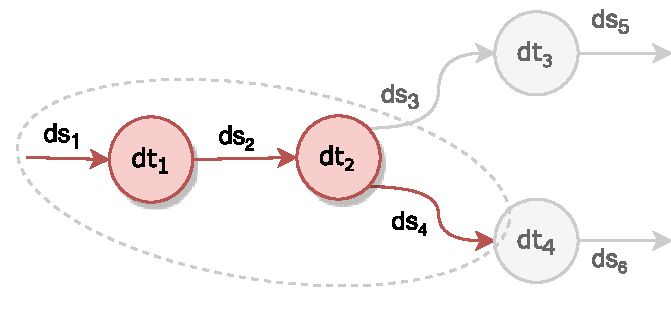
\includegraphics[width=\textwidth]{img/example-query-dataflow-1}
    \caption[Caminho obtido na consulta do exemplo \#1]{Caminho de conjuntos de dados obtido na consulta do exemplo \#1: \(\{ds_{1} \rightarrow ds_{2} \rightarrow ds_{4}\}.\)}%
    \label{fig:example-query-dataflow-1}
\end{figure}

\begin{minipage}[c]{0.95\textwidth}
\begin{lstlisting}[language=sql,label={lst:example-query-output-1},caption={[Código SQL gerado no exemplo~\#1]Código SQL gerado pela função \texttt{generateSqlQuery} no exemplo~\#1.}]
SELECT %$ds_{1}.da_{1}$%, %$ds_{1}.da_{2}$%, %$ds_{2}.da_{1}$%, %$ds_{2}.da_{2}$%, %$ds_{4}.da_{3}$%
FROM %$ds_{1}$%,%$ds_{2}$%,%$ds_{4}$%
WHERE %$ds_{1}.\textup{taskid}\_dt_{1} = ds_{2}.\textup{taskid}\_dt_{1}$% and -- mapeamento físico
      %$ds_{2}.\textup{taskid}\_dt_{2} = ds_{4}.\textup{taskid}\_dt_{2}$% and -- mapeamento físico
      %$ds_{1}.da_{1} = ds_{2}.da_{1}$% and           -- mapeamento lógico
      %$ds_{1}.da_{1} > 100$%;                 -- seleção provida pelo usuário
\end{lstlisting}
\end{minipage}

\begin{table}[!htb]
    \centering
    \begin{tabular}{c|c|c|c|c}
\textbf{ds\textsubscript{1}.da\textsubscript{1}} & \textbf{ds\textsubscript{1}.da\textsubscript{2}} & \textbf{ds\textsubscript{2}.da\textsubscript{1}} & \textbf{ds\textsubscript{2}.da\textsubscript{2}} & \textbf{ds\textsubscript{4}.da\textsubscript{3}} \\ \hline
200              & falso            & 200              & -45              & bravo            \\
200              & falso            & 200              & -45              & charlie          \\
300              & verdadeiro       & 300              & 42               & bravo            \\
300              & verdadeiro       & 300              & 42               & charlie         
    \end{tabular}
    \caption[Resultados obtidos com a consulta em SQL do exemplo \#1]{Resultados obtidos com a consulta em SQL do exemplo \#1.}
    \label{tab:example-query-results-1}
\end{table}